% MA211 - Lecture 08
\documentclass[pdftex, xcolor=pdftex, dvipsnames,handout]{beamer}

\usetheme{MA211}
\usepackage{thumbpdf}
\usepackage{wasysym}
%\usepackage{ucs}
\usepackage[utf8]{inputenc}
\usepackage{pgf,pgfarrows,pgfnodes,pgfautomata,pgfheaps,pgfshade}
\usepackage{verbatim}

\usepackage{eurosym}
\usepackage{euler}

\usepackage{calc}               % Simple computations with LaTeX variables
%\usepackage[hang]{caption2}     % Improved captions

\usepackage{graphicx}           % Standard graphics package

\usepackage{amsmath, amsthm, amssymb}


\newcommand{\fquad}{\mbox{\qquad}}
\newcommand{\bull}{$\bullet$ }

\newcommand {\I} {\mathcal I}
\newcommand {\calI} {\mathcal I}
\def\disint{\displaystyle\int}

\DeclareMathOperator{\D}{d}
\newcommand{\dydx}{\frac{\D y}{\D x}}

%\definecolor{gray}{rgb}{0.69, 0.69, 0.69} \newcommand{\gray}[1]{\textcolor{gray}{#1}}
\definecolor{dogreen}{rgb}{0.33, 0.42, 0.18} \newcommand{\dogreen}[1]{\textcolor{dogreen}{#1}}
\definecolor{maroon}{rgb}{.5,0.2,0.2}\newcommand{\maroon}[1]{\textcolor{maroon}{#1}}
\definecolor{greena}{rgb}{.1,0.581,0.1}\newcommand{\greena}[1]{\textcolor{greena}{#1}}

\definecolor{blue4}{rgb}{0,0,.545}
\newcommand{\Blue}[1]{\textcolor{blue}{#1}}
\newcommand{\Red}[1]{\textcolor{red}{#1}}
\definecolor{pink}{rgb}{1.,0.75,0.8}
\definecolor{darkred}{rgb}{0.5,0.0,0.0}
\definecolor{darkgreen}{rgb}{0,0.3,0.3}
\definecolor{purple}{rgb}{0,0.3,0.3}
\definecolor{darkblue}{rgb}{0.0, 0.0, .5}
\definecolor{dpurple}{rgb}{.3,.0,.3}
\newcommand{\Green}[1]{\textcolor{darkgreen}{#1}}
\newcommand{\DRed}[1]{\textcolor{darkred}{#1}}
\newcommand{\DBlue}[1]{\textcolor{darkblue}{#1}}
\newcommand{\Purple}[1]{\textcolor{dpurple}{#1}}
\newcommand{\Emph}[1]{\textcolor{darkred}{\textbf{\it #1}}}
\newcommand{\remph}[1]{\textcolor{darkred}{\textbf{\emph{#1}}}}
\newcommand{\bemph}[1]{\textcolor{darkblue}{\textbf{\emph{#1}}}}
\newcommand{\gemph}[1]{\textcolor{darkgreen}{\textbf{\emph{#1}}}}
\newcommand{\Bf}[1]{\textcolor{darkblue}{\textbf{#1}}}
\newcommand{\Gf}[1]{\textcolor{darkgreen}{\textbf{#1}}}
\newcommand{\Rf}[1]{\textcolor{red}{\textbf{#1}}}
\newcommand{\Rmf}[1]{\textcolor{red}{\mathbf{#1}}}

\newcommand{\Conj}[1]{\overline{#1}}

\newcommand{\code}[1]{\textcolor{darkblue}{\texttt{\textbf{#1}}}}
\newcommand{\icode}[1]{{\blue\texttt{\textbf{\emph{#1}}}}}
\newcommand{\gcode}[1]{{\Green{\texttt{\textbf{\emph{#1}}}}}}
\newcommand{\out}[1]{\texttt{\emph{\textbf{\Green{#1}}}}}





\newenvironment{vminipage}%
{\begin{Sbox}\begin{minipage}\begin{small}\begin{verbatim}}%
{\end{verbatim}\end{small}\end{minipage}\end{Sbox}\fbox{\TheSbox}}

\newenvironment{nminipage}%
{\begin{Sbox}\begin{minipage}}%
{\end{minipage}\end{Sbox}\fbox{\TheSbox}}


\let\Arg\relax\DeclareMathOperator{\Arg}{\mathtt{Arg}}
\let\Arg\relax\DeclareMathOperator{\e}{\mathtt{e}}

\newcommand {\AND} {\wedge}
\newcommand {\OR} {\vee}
\newcommand {\NOT} {\neg}
\newcommand {\IMPLIES} {\rightarrow}
%\newcommand {\IFF} {\leftrightarrow}
\renewcommand {\iff} {\Leftrightarrow}
\newcommand {\NAND} {\uparrow}
\newcommand {\NOR} {\downarrow}
\newcommand {\XOR} {\otimes}

\newenvironment{citemize}% Colour items
{\begin{description}}%
{\end{description}}

\newcommand {\maroonitem}{\item[\maroon{$\bullet$}]}

\newcommand {\gitem} {\item {\includegraphics[width=.4cm,angle=-10]{img/green-bullet-on-white.ps}}}
\newcommand {\ritem} {\item {\includegraphics[width=.4cm,angle=-10]{img/red-bullet-on-white.ps}}}
\newcommand {\yitem} {\item {\includegraphics[width=.4cm,angle=-10]{img/yellow-bullet-on-white.ps}}}
\newcommand {\bitem} {\item {\includegraphics[width=.4cm,angle=-10]{img/blue-bullet-on-white.ps}}}

\newcommand {\greenitem} {\item {\includegraphics[width=.4cm,angle=-10]{img/green-bullet-on-white.ps}}}
\newcommand {\reditem} {\item {\includegraphics[width=.4cm,angle=-10]{img/red-bullet-on-white.ps}}}
\newcommand {\yellowitem} {\item {\includegraphics[width=.4cm,angle=-10]{img/yellow-bullet-on-white.ps}}}
\newcommand {\blueitem} {\item {\includegraphics[width=.4cm,angle=-10]{img/blue-bullet-on-white.ps}}}

\newcommand {\eq}[1]%
  {$\DBlue{#1}$}
\newcommand {\eqd}[1]%
  {$\displaystyle\DBlue{#1}$}
%\newcommand{\eq}[1]{\boldmath \DBlue{$#1$}}


\newcommand {\csf}{\centerslidesfalse}
\newcommand {\cst}{\centerslidestrue}

\newcommand {\vecii}[2] {   \big(\begin{smallmatrix} #1 \\ #2 \end{smallmatrix}\big)}
\newcommand{\atwo}[2]{\left(\!\!\begin{array}{c} #1 \\ #2 \end{array}\!\!\right)}


\newcommand{\C}{\mathbb{C}}
\newcommand{\Q}{\mathbb{Q}}
\newcommand{\R}{\mathbb{R}}
\newcommand{\N}{\mathbb{N}}
\newcommand{\Z}{\protect\mathbb{Z}}  % protect for index.
\newcommand {\Rs}{ \mathbb{R}}
\newcommand {\Cs}{ \mathbb{C}}
\newcommand {\Rnn}{ \mathbb{R}^{n \times n}}
\newcommand {\Rn}{ \mathbb{R}^{n}}


\newcommand{\mblock}{%
\setbeamercolor*{block title}{bg=maroon,fg=white}
\setbeamercolor*{block body}{bg=white,fg=maroon}
}%

\newcommand{\bblock}{%
\setbeamercolor*{block title}{bg=Steel,fg=white}
\setbeamercolor*{block body}{bg=Mylightgray,fg=Steel}
}%

\newcommand{\gblock}{%
\setbeamercolor*{block title}{bg=Green,fg=white}
\setbeamercolor*{block body}{bg=Mylightgray,fg=darkgreen}
}%


\newcommand{\rblock}{%
\setbeamercolor*{block title}{bg=Red,fg=white}
\setbeamercolor*{block body}{bg=white,fg=Black}
}%


\newcommand{\TakeNotes}{
\includegraphics[width=2cm]{TakeNote}}

\def\eps{\varepsilon}
\newcommand {\del}[2]{ {\frac{\partial #1}{\partial #2}}}
\newcommand {\x}[1]{x^{[#1]}}
\newcommand {\delx}{ {\frac{\partial}{\partial x}}}
\newcommand {\delt}{ {\frac{\partial}{\partial t}}}
\newcommand {\dely}{ {\frac{\partial}{\partial y}}}
\newcommand {\ith}{{(i)}}
\renewcommand {\vec}[1]{ {\boldsymbol{#1}}}
\newcommand {\Oh} {\mathcal O}
\newcommand {\Err} {\mathcal E}
%\newcommand {\th} {\mathrm{th}}
\DeclareMathOperator{\fl}{fl}
\DeclareMathOperator{\sign}{sign}
\DeclareMathOperator{\Cond}{Cond} 
\DeclareMathOperator{\cond}{cond}
\DeclareMathOperator{\diag}{diag} 
\DeclareMathOperator{\sym}{sym} 
\DeclareMathOperator{\Trace}{Trace}
\DeclareMathOperator{\E}{e}

\newcommand {\Rsym}{{ \mathbb{R}^{n \times n}_\mathrm{sym}}}

\newcommand {\st} {\mathrm{st}}
\newcommand {\nd} {\mathrm{nd}}


\parskip .25cm


\theoremstyle{definition}
\newtheorem{exercise}{Exercise}[section]
\newtheorem{method}{Method}[section]

\newcommand{\Header}[1]{\begin{center}{\Large \Bf{#1}}\end{center}}

\subtitle{MA211}
\title{Lecture 8: Hyperbolic Functions}

\author{Dr Niall Madden}

\date{\Large Wed, 01 October  2008}


\begin{document}


\frame{

\begin{block}{}
\begin{center}
{\large \insertsubtitle}

\vspace{.1cm}

\begin{Large}
\textbf{\inserttitle}
\end{Large}

\vspace{.15cm}

% {\footnotesize \insertauthor}

\vspace{.3cm}

{ {\insertdate}}
\end{center}
\end{block}


\vspace{-0.25cm}
\begin{center}
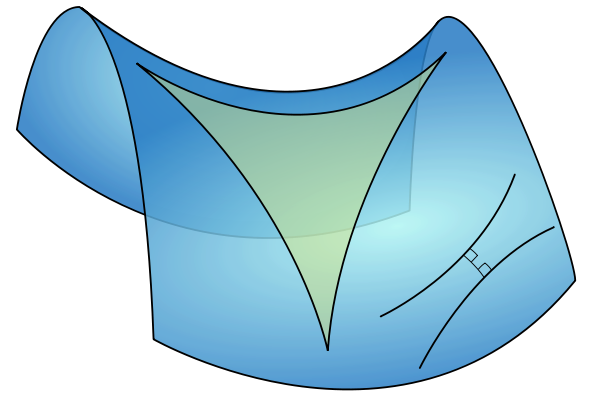
\includegraphics[height=4cm]{images/Hyperbolic}

\end{center}
}


\frame{

\Header{Reminder: Problem Set 1}

Deadline for the homework exercises from Problem Set 1 is
\Emph{11am, Monday, Oct 6th}.



}

\frame{
  \frametitle{In today's class}

%\begin{columns}[c]
%\column{0.5\textwidth}
%\begin{small}
 \tableofcontents
%\end{small}

%\column{0.5\textwidth}
For more details, see \Bf{Sections 1.6, 3.5 and  3.11} of Stewart.

%\end{columns}

}


\renewcommand{\arraystretch}{2}

\frame{
\frametitle{Last week... The Natural Logarithm}

Last week we define the ``\Emph{natural logarithm of \eq{x}}'', usually written
 \eq{\ln(x)}, as  follows: Let \eq{A} be the area of the region from
 \eq{t=1} to 
\eq{t=x}  between the curve 
\eq{1/t} and the \eq{t}-axis. 
\begin{center}
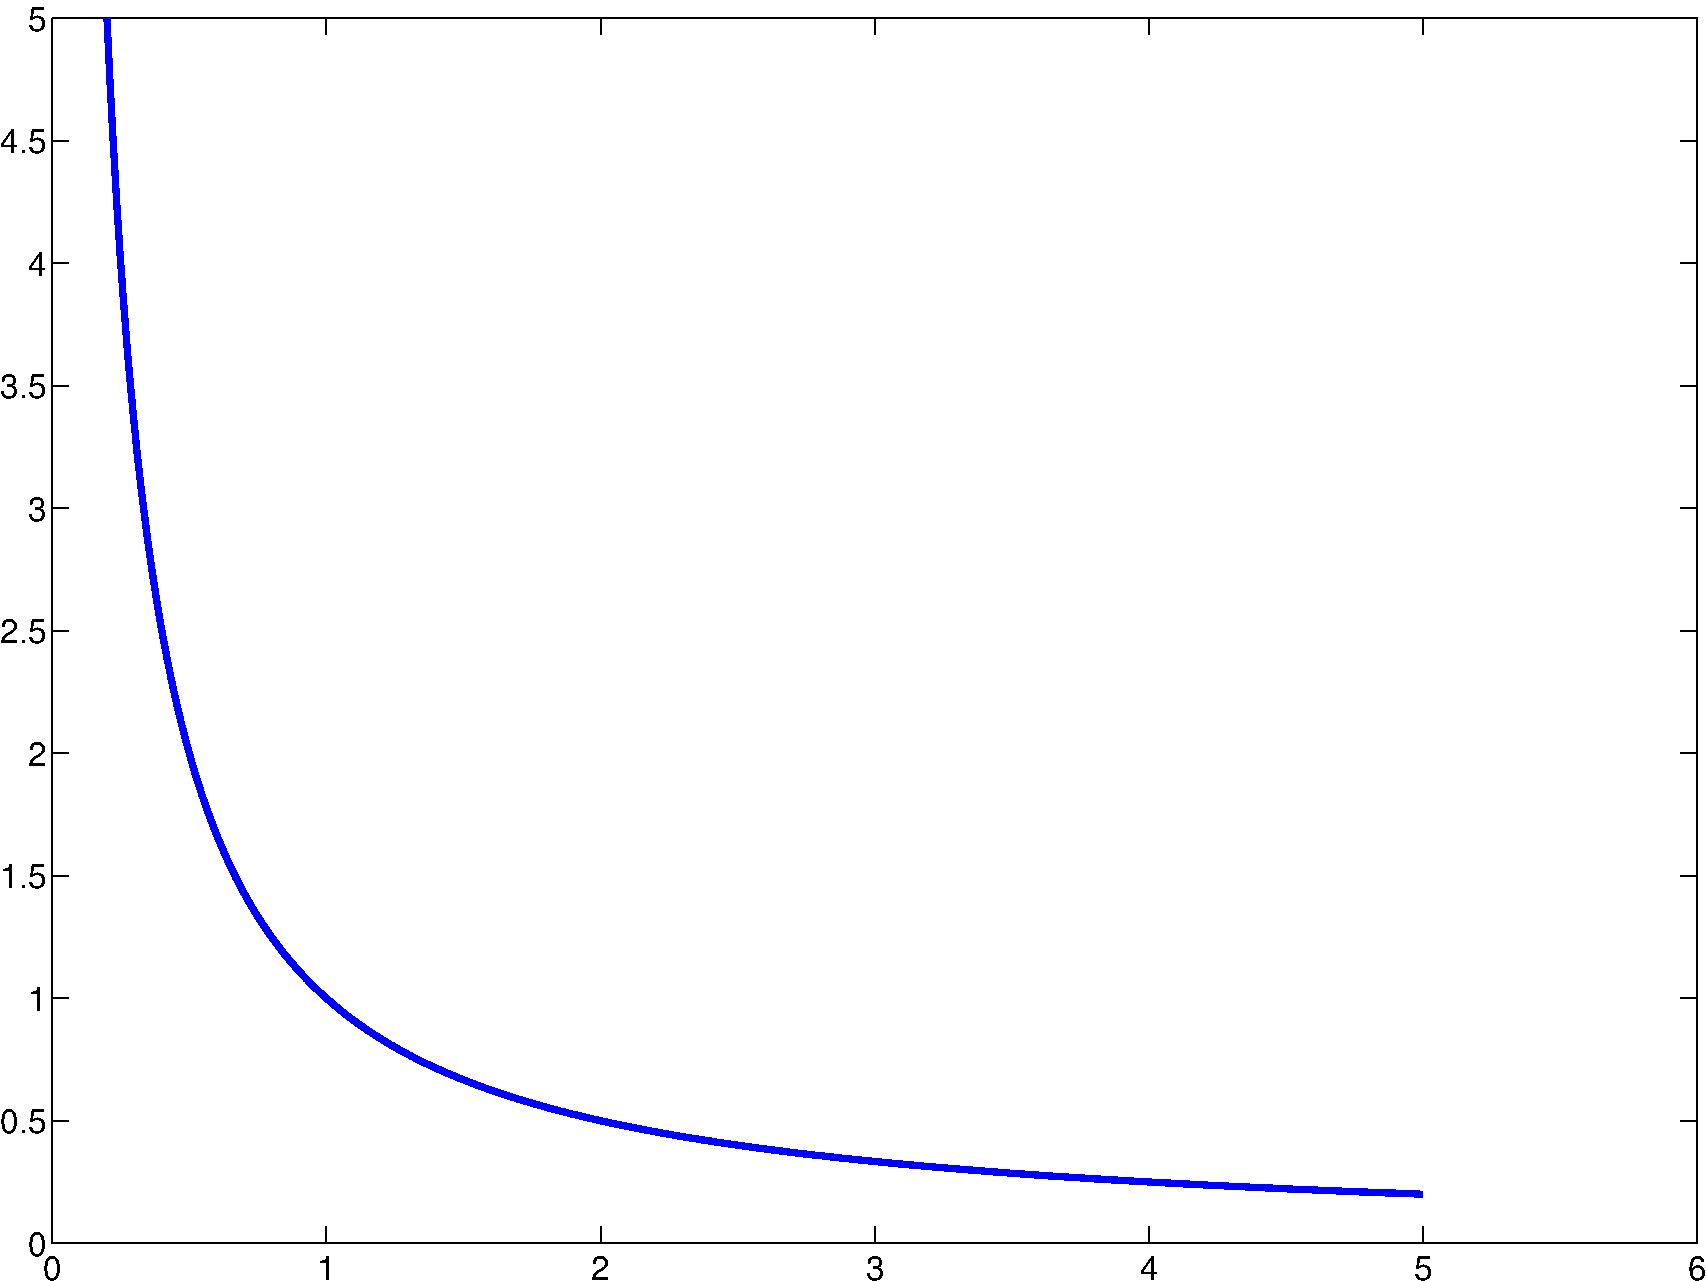
\includegraphics[width=7cm]{images/OneOverX}
\end{center}
}


\frame{

Then we define \eq{\ln x} as
\[
\ln(x) = \begin{cases}
A, & \text{ for } x \geq 1\\
-A, & \text{ for } 0< x < 1.
\end{cases}
\]

\begin{center}
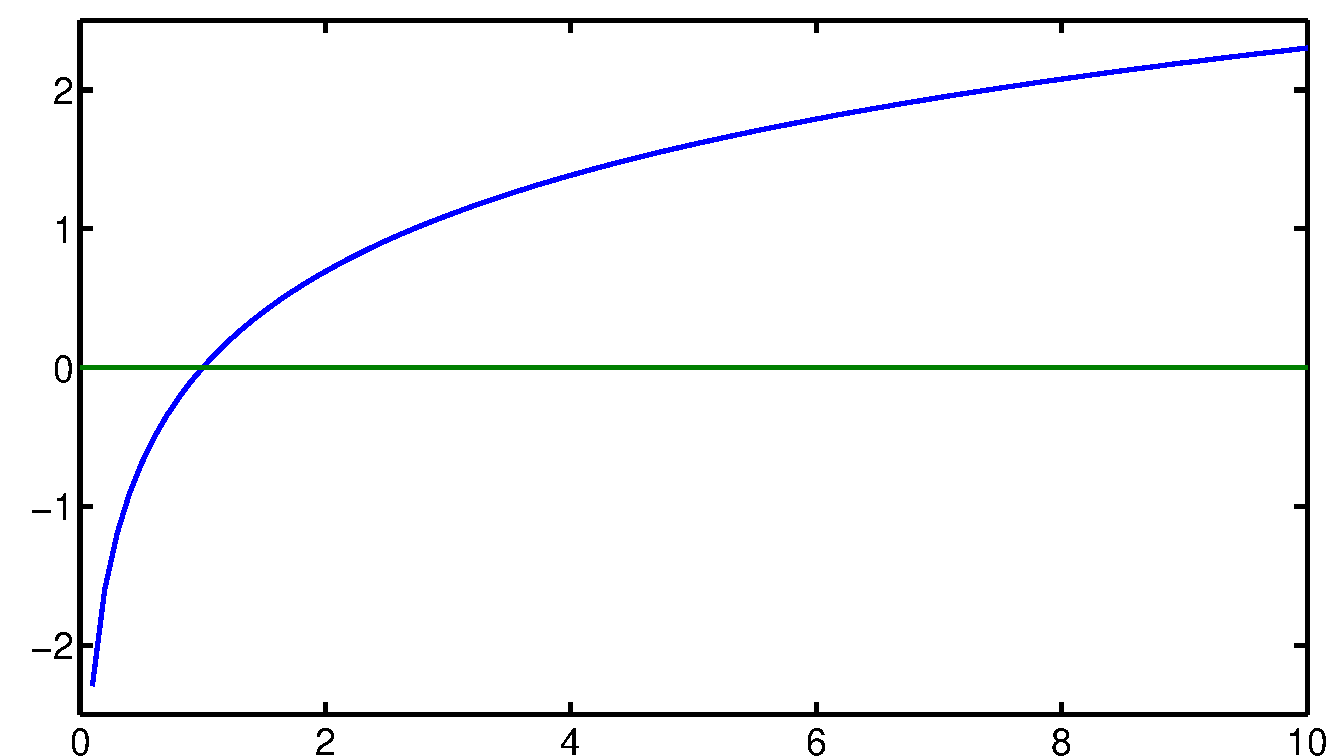
\includegraphics[width=7cm]{images/ln}
\end{center}

}

\frame{

We then proved that, if \eq{x>0} then
\[
\frac{d}{dx}\ln (x) = \frac{1}{x}.
\]

Equivalently:
\[
\int \frac{1}{x} dx = \ln(x) + C
\]

\pause
Although it is not defined in the same way as  other logarithmic
functions, the 
Natural Log enjoys the same important properties:
\begin{block}{}
\begin{enumerate}[(i)]
\item  \eq{\ln (xy) = \ln(x) + \ln(y)}
\hfill 
(ii) \eqd{\ln\big(\frac{1}{x}\big) = -\ln x}

\vspace{.3cm}
\item[(iii)] \eqd{\ln\big(\frac{x}{y}\big) = \ln x - \ln y}
\hfill 
(v) \eq{\ln \big(x^y) = y \ln x}
\end{enumerate}
\end{block}

}

\section{Recall: The exponential function}
\frame{
Next we defined the inverse of the \Bf{Exponential Function} as the
inverse of the Natural Logarithmic Function

\begin{definition}[Exponential Function $\exp(x)$]
The function \eq{\exp:(-\infty, \infty)\to(0,\infty)} is the inverse
of the natural log function \eq{\ln:(0,\infty)\to(-\infty, \infty)}:
\[ y = \ln(x) ~~ \Longleftrightarrow ~~ x = \exp(y). \]
\end{definition}

\begin{center}
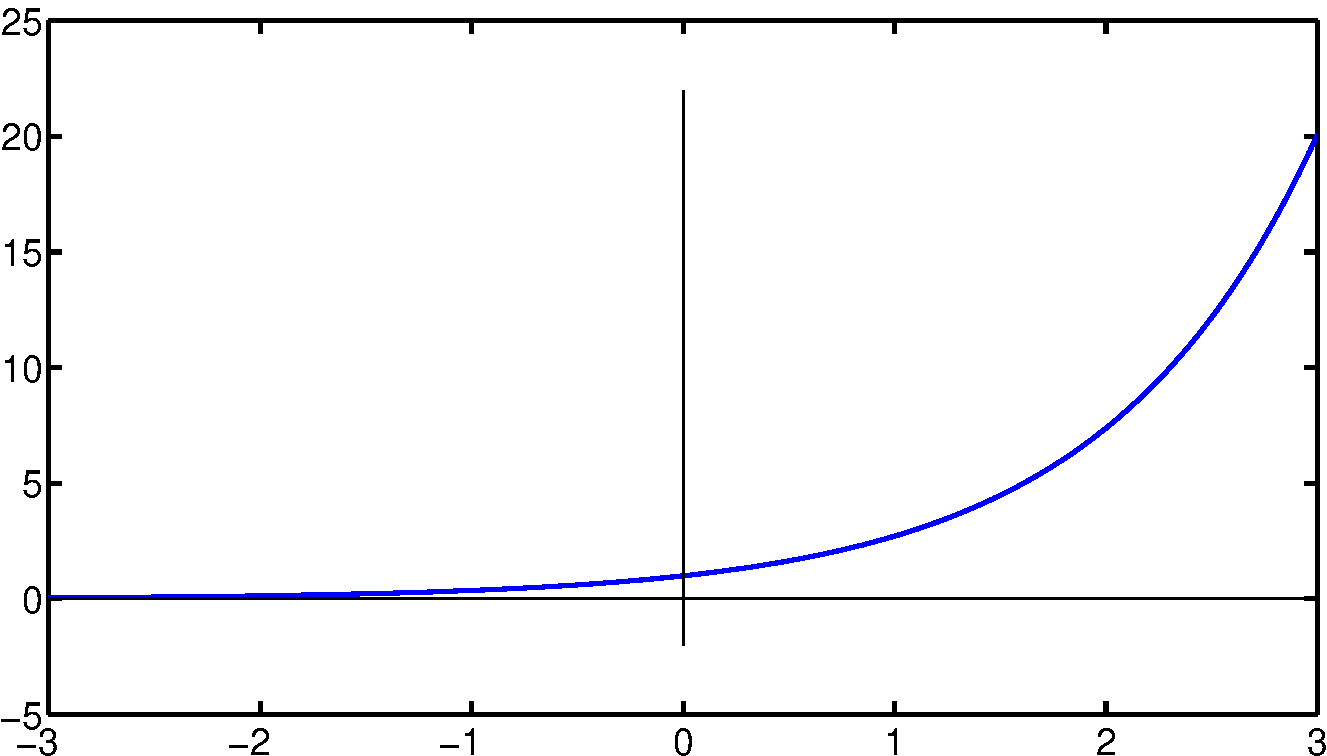
\includegraphics[width=6.5cm]{images/exp}
\end{center}

}

\frame{

By definition:
\[
\ln(\exp(x)) = x \qquad \text{ for all } x\in\R
\]
and
\[
\exp(\ln(x)) = x \qquad \text{ for all } x\in\R^+=(0,\infty)
\]

}

\subsection{Properties}
\frame{
From the properties of \eq{\ln(x)}, we can deduce that the $\exp$
function satisfies the usual properties on the exponential function $y=a^x$.
\begin{block}{}
\begin{enumerate}[(i)]
\item \eq{\exp(x+y) = \exp(x)\exp(y)}
\hfill
(ii) \eqd{\exp(-x) = \frac{1}{\exp(x)}}

\vspace{1.3cm} 

\item \eqd{\exp(x-y) = \frac{\exp(x)}{\exp(y)}}
\hfill
(iv) \eq{\exp(x)^y = \exp(xy)}

\end{enumerate}
\end{block}




Perhaps the most important property:


\begin{alertblock}{}

\[ \frac{d}{dx}e^x = e^x.\]
So the exponential function is its own derivative!
\end{alertblock}

}



\frame{

Because the derivative of \eq{e^x} is \eq{e^x}, we also get:
\[ \int e^x dx = e^x +C \]


\begin{example}
 Calculate the integral of \eq{f(x) =  A e^{Bx}},  where \eq{A} and \eq{B} are constants.
\end{example}


\Bf{Solution:}
\eqd{\int A e^{Bx} dx = A \int  e^{Bx} dx = \frac{A}{B} e^{Bx} + C}.


}


\frame{

\begin{example}
Solve the Initial Value Differential Equation
\[
f'(x) - f(x) =0; f(0)=2;
\]
\end{example} 
\Bf{Solution:}

\vspace{2.3cm}

}


\section{Inverse Trigonometric functions}
\subsection{$\sin^{-1}(x)$}

\frame{
Recall the function \eq{\sin:(-\infty, \infty) \to [-1,1]}:
\begin{center}
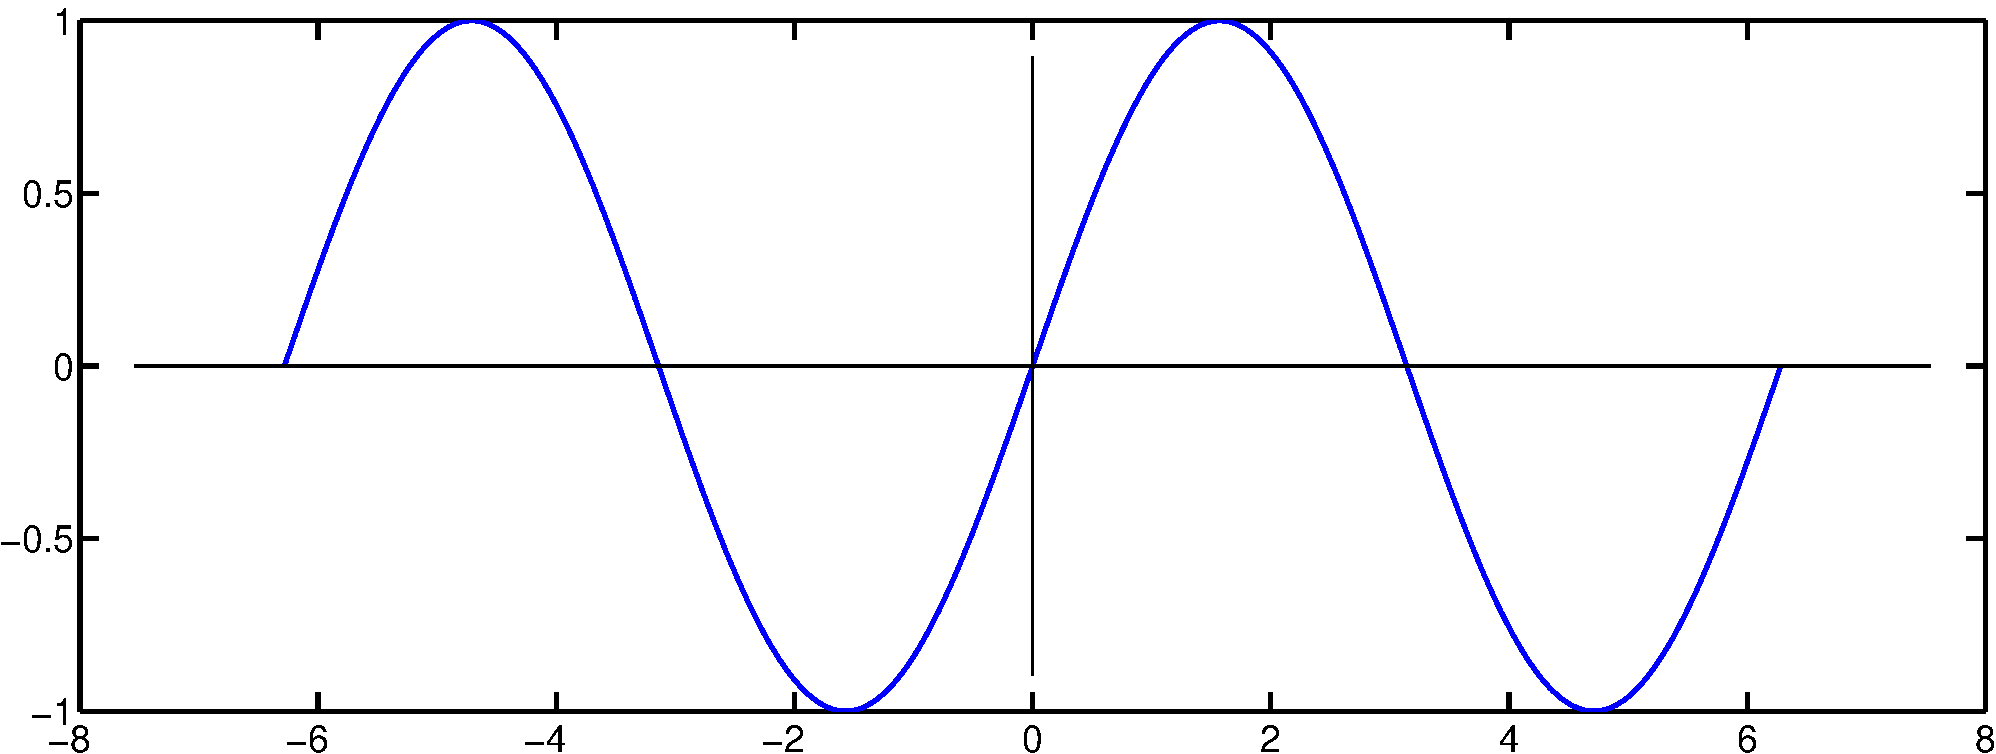
\includegraphics[width=9cm]{images/sin}
\end{center}

This function is \Emph{not} invertible, because it is not one-to-one.
However, if we restrict the domain to $[-\frac{\pi}{2},
\frac{\pi}{2}]$, then it is invertible.

}

\rblock
\frame{
\begin{columns}[c]
\column{0.5\textwidth}
\begin{block}{Inverse $\sin$ function}
The inverse of the \eq{\sin} function on $[-\pi/2, \pi/2]$ is
denoted \eq{\sin^{-1}(x)} or \eq{\arcsin(x)}
\[ y = \sin(x) \Longleftrightarrow x = \sin^{-1}(y).\]
\end{block}

\vspace{1cm}

\pause 
The notation $\arcsin$ is still often used text books, but we'll use
\eq{\sin^{-1}}.  Take care not to confuse this with $1/\sin(x)$.

\column{0.5\textwidth}

\begin{center}
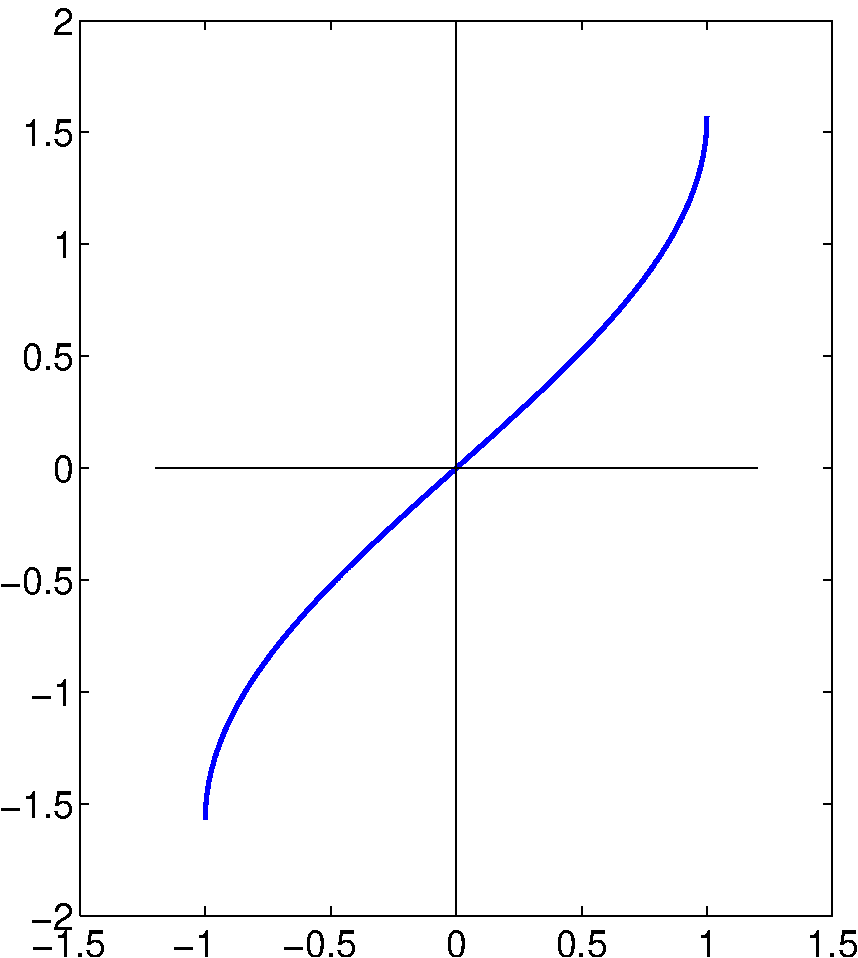
\includegraphics[width=5cm]{images/asin}
\end{center}


\end{columns}
}

\frame{
\begin{example}
Simplify \eqd{\tan\big( \sin^{-1}(x)\big)}.
\end{example}


\vspace{3cm}
}

\subsection{$\sin^{-1}, \cos^{-1}$ and $\tan^{-1}$}

\frame{

We can also define the inverse of the \eq{\cos} and \eq{\tan}
functions. 

\begin{exercise}[Q8.1]
\begin{enumerate}[(i)]
\item Show that \eqd{\cos (\tan^{-1}(x)) = \frac{1}{\sqrt{1+x^2}}}.
~

\item Simplify the expression \eq{\sin(\tan^{-1}(x))}
~

\item Simplify the expression \eq{\cos(2\tan^{-1}(x))}
\end{enumerate}
\end{exercise}
}


\frame{

The derivatives of the inverse trig functions are

\begin{center}
\begin{tabular}{c|c}
$\boldmath{\alert{ f(x)}}$ & $\displaystyle \boldmath \alert{\frac{d}{dx} f(x) } $\\ \hline
$\sin^{-1}(x)$ &\\ \hline
$\cos^{-1}(x)$ &\\ \hline
$\tan^{-1}(x)$ & 
\end{tabular}
\end{center}
(See p41 in the Mathematical Tables).

However, we \alert{need} to be able to  work these out using the \Emph{Chain Rule}.
}

\frame{

\begin{example}
Use the Chain Rule, and that \eq{\cos^2(x) + \sin^2(x) = 1} to find the derivative of \eq{y = sin^{-1}(x)}
\end{example}


\vspace{4cm}
}

\frame{
\begin{exercise}[Q8.2]
 Show that  
\begin{enumerate}[(i)]
\item $\displaystyle \frac{d}{dx} \big(\sin^{-1}(x)\bigg) =
  \frac{1}{\sqrt{1 - x^2}}$.
\item 
$\displaystyle \frac{d}{dx} \big(\cos^{-1}(\frac{x}{a})\bigg) =
  \frac{-1}{\sqrt{a^2 - x^2}}$.

\item 
$\displaystyle \frac{d}{dx} \big(\tan^{-1}(\frac{x}{a})\bigg) =
  \frac{1}{{a^2 + x^2}}$.
\end{enumerate}
\end{exercise}
Hint: Use that 
\begin{itemize}
\item $\cos^2 (x) + \sin^2(x) =1$,
\item \eq{\sec(x) = 1/\cos(x)},
\item $\sec^2(x) = 1 + \tan^2(x)$.
\end{itemize}
}

\section{Euler Formula}

\frame{
For complex numbers, it is possible to express \eq{e^x} in terms of
\eq{\sin} and \eq{\cos}:
\begin{alertblock}{}
\[
e^{i x} = \cos(x) + i \sin(x), \quad \text{ where } i =\sqrt{-1}.
\]
This is known as \Emph{Euler's Formula}.
\end{alertblock}



}

\frame{
\begin{example}
Use that
\[
\cos(x) = \frac{1}{2}\big(e^{ix} + e^{-ix}\big)
\]
to find \eq{\frac{d}{dx}\cos(x)}.
\end{example}
\Bf{Solution:}
\vspace{3cm}

}


\frame{


\begin{exercise}[Q8.3]
 Use the Euler formula to show the following:
\begin{enumerate}[(i)]
\item \eqd{\sin(x) = \frac{-i}{2}\big(e^{ix} - e^{-ix}\big),}

~

\item \eqd{\frac{d}{dx}\sin(x) = \cos(x)}

~

\item \eqd{\int \sin(x) = -\cos(x)+C}

~

\item \eqd{\sin^2(x) + \cos^2(x) = 1}
\end{enumerate}
\end{exercise}
}

\bblock
\section{The Hyperbolic Functions}

\frame{

From Euler's formula, we can get the following definitions of 
\eq{\sin} and \eq{\cos}
\begin{block}{}
\[ 
 \cos(x) = \frac{1}{2}\big(e^{ix} + e^{-ix}\big),
\quad 
\text{ and } 
\quad
\sin(x) = \frac{-i}{2}\big(e^{ix} - e^{-ix}\big).
\]
\end{block}

Based on these, can define their \Emph{Hyperbolic} analogs...

}

\frame{


\rblock
\begin{definition}[Hyperbolic Functions]
  The \Bf{Hyperbolic cosine and sine functions} are defined as
\[
\cosh(x) = \frac{1}{2}\big({e^x - e^{-x}}\big), 
\quad 
\text{ and } 
\quad
\sinh(x) = \frac{1}{2}\big({e^x - e^{-x}}\big), 
\]
\end{definition}
\begin{center}
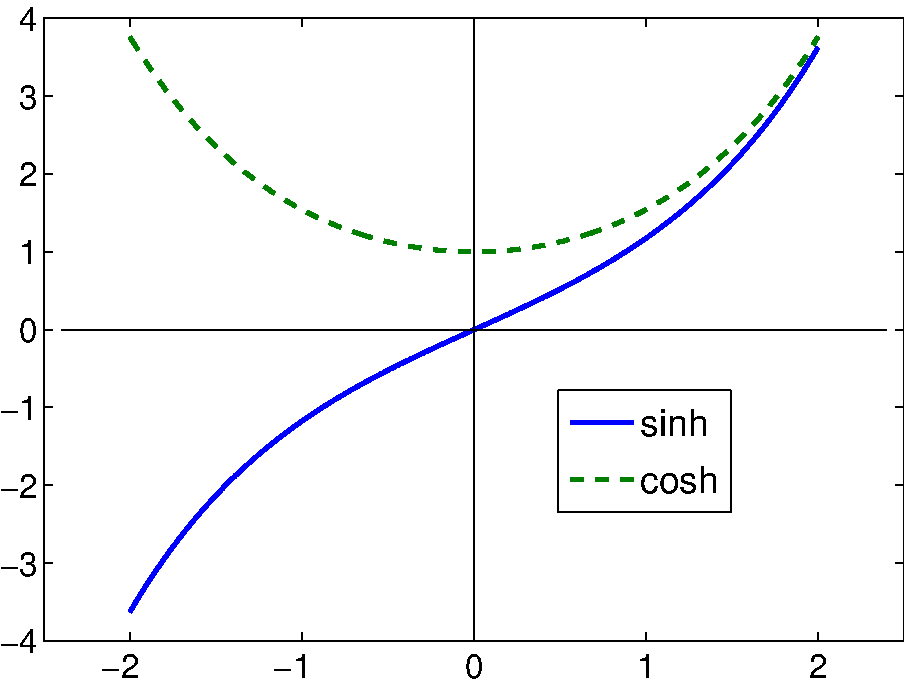
\includegraphics[width=6cm]{images/sinh}
\end{center}

}





\subsection{Derivatives}
\frame{

\gblock
\begin{block}{Derivative of $\sinh(x)$}
\[ \frac{d}{dx}(\sinh x) = \cosh x \]
\end{block}

\Bf{Proof:}

\vspace{3cm}

\rblock
\begin{exercise}
Show that 
\[ \frac{d}{dx} (\cosh x) = \sinh x \]
\end{exercise}

}

\subsection{Inverses}
\frame{

\gblock
\begin{block}{}%{Derivative of $\sinh(x)$}
Express \eq{\sinh^{-1}(x)} in terms of logarithms.
\end{block}

\Bf{Answer:}

\vspace{3cm}

\rblock
\begin{exercise}
Show that 
\[ \cosh^{-1}x = \ln \big( x + \sqrt{x^2-1}\big)\]
\[ \tanh^{-1}x = \frac{1}{2}\ln \big( \frac{1+x}{1-x}\big)\]
\end{exercise}

}

\end{document}
\subsection{Examples}

\frame{
\begin{example}[Q1 (b), Semester 1, 05/06]
\begin{enumerate}[<+->][(i)]
\item Define the hyperbolic functions \eq{y=\cosh(x)} and  \eq{y=\sinh(x)}
\item What is the largest possible domain for \eq{y=\cosh(x)}? What is the largest possible domain for \eq{y=\cosh^{-1}(x)}?
\item Sketch the graphs of \eq{y=\cosh(x)} and \eq{y=\cosh^{-1}(x)}
\item Prove that \eq{\cosh(2x) = \cosh^2(x) + \sinh^2(x)}
\item Prove that 
\[
\frac{d}{dx}\bigg( \cosh^{-1}\frac{x}{a}\bigg) = \frac{1}{\sqrt{x^2 -
    a^2}}.
\]
\end{enumerate}
\end{example}
Note: for part (v), you'll need to use that \eq{\cosh y = \sqrt{1 + \sinh^2 y}}. This
comes from the fact that \eq{\cosh^2 y - \sinh^2y=1}.

}

\end{document}

\frame{


\begin{block}{}
The \eq{\tanh} and \eq{cotanh} functions can be defined 
\[ \tanh x = \frac{\sinh x}{\cosh x}, \qquad 
\coth x = \frac{1}{\tanh x} = \frac{\cosh x}{ \sinh x}. \]
\end{block}
\begin{center}
\includegraphics[width=5.6cm]{Matlab/tanh}
\end{center}


}
\rblock
\frame{

\begin{exercise}

Recall that
\[
\cos^2 x + \sin^2 x = 1.
\]

Show that
\[
\cosh^2 x - \sinh^2 x =1.
\]

\end{exercise}
}


\frame{
The previous slide highlights a difference between the hyperbolic and
trig functions. Nonetheless, they have much in common:


\begin{example}
\eq{ \cosh (x+y) = \cosh x \cosh y + \sinh x \sinh y }
\end{example}
(To show this is true, we repeatedly use that \eq{e^a e^b=e^{a+b}}).\\
First, from the definition of \eq{\cosh}, 
\[
\cosh(x+y) = \frac{1}{2}\big( e^{x+y} + e^{-x-y}\big).
\]
Then \eq{\cosh x \cosh y + \sinh x \sinh y =}
\begin{gather*}
\frac{1}{4}\big[ (e^x + e^{-x})(e^y + e^{-y}) + (e^x - e^{-x})(e^y -
e^{-y})\big] =
\\
\frac{1}{4}\big[ e^{x+y} + e^{x-y} + e^{-x+y} + e^{-x-y} + e^{x+y} -
e^{-x+y} - e^{x-y} + e^{-x-y}\big] =
\\
\frac{1}{4}\big[ 2e^{x+y} + 2 e^{-x-y}\big]
= \frac{1}{2}\big[ e^{x+y} +  e^{-x-y}\big].
\end{gather*}

}

\frame{
\begin{exercise}
Show that
\[ \sinh (x+y) = \sinh x \cosh y + \cosh x \sinh y.\]
\end{exercise}


}


%\frame{
%\begin{example}
% Differentiate $\tanh x$.
%\end{example}
%\Bf{Solution:}
%}


\section{Differential Equations}

\frame{
Now that we have the exponential, logarithmic, trigonometric and
hyperbolic functions at our disposal, we can solve some differential
equations.


The DEs that we'll look at now are of 
\Header{2nd Order, Constant Coefficient, Homogeneous type.}

\begin{example}
\[\frac{d^2y}{dx^2} + \frac{dy}{dx} - 2y = 0 \Longleftrightarrow 
y''(x) + y'(x) -2y(x) =0.\]
\end{example}

}

\frame{
\begin{example}
\[\frac{d^2y}{dx^2} + \frac{dy}{dx} - 2y = 0 \Longleftrightarrow 
y''(x) + y'(x) -2y(x) =0.\]
\end{example}

Suppose the solution is \eq{y(x) = e^{rx}}. Then \eq{y'(x) = re^{rx} =
  ry(x)} and \eq{y''(x) = r^2e^{rx} = r^2y(x)}.

Substituting into the equation we get that
\[
r^2 e^{rx} + re^{rx} - 2 e^{rx} =0.
\]
Dividing across by \eq{e^{rx}}, we get a quadratic equation for
\eq{r}:
\[
r^2 + r -2 =0.
\]
This has two solutions: \eq{r=1} and \eq{r=-2}. 
}






\end{document}



\frame{

\begin{block}{}
The \eq{\tanh} and \eq{cotanh} functions can be defined 
\[ \tanh x = \frac{\sinh x}{\cosh x} \]
\[ \coth x = \frac{1}{\tanh x} = \frac{\cosh x}{ \sinh x}. \]
\end{block}
\begin{center}
\includegraphics[width=5.6cm]{images/tanh}
\end{center}




}
\rblock
\frame{

\begin{exercise}

Recall that
\[
\cos^2 x + \sin^2 x = 1.
\]

Show that
\[
\cosh^2 x - \sinh^2 x =1.
\]

\end{exercise}
}


\frame{
The previous slide highlights a difference between the hyperbolic and
trigonometric functions. Nonetheless, they have much in common:


\begin{itemize}[<+->]
\item $\cosh (x+y) = \cosh x \cosh y + \sinh x \sinh y$
\item $\sinh (x+y) = \sinh x \cosh y + \cosh x \sinh y$
\end{itemize}

\Bf{Example:}

\vspace{2cm}

}

\frame{

\begin{theorem}
\begin{itemize}
\item $\frac{d}{dx}(\sinh x) = \cosh x$
\item $\frac{d}{dx} (\cosh x) = \sinh x$
\end{itemize}
\end{theorem}

\Bf{Proof:}

\vspace{3cm}


}

\frame{
\begin{example}
 Differentiate $\tanh x$.
\end{example}
\Bf{Solution:}


\vspace{2cm}

}

% \frame{

% \begin{example}
% Which of the following functions:
% \begin{enumerate}[(i)]
% \item \eqd{y(x) = \sin(x)}
% \item \eqd{y(x) = \cos(x)}
% \item \eqd{y(x) = \exp(x)}
% \item \eqd{y(x) = \exp(-x)}
% \end{enumerate}
% are solutions to the differential
% equations
% \begin{enumerate}[(a)]
% \item \eqd{y'(x) + y(x)=0},
% \item \eqd{y'(x) - y(x)=0},
% \item \eqd{y''(x) + y(x)=0},
% \item \eqd{y''(x) - y(x)=0},
% \end{enumerate}
% \end{example}

% \pause \alert{Need a solution to (d)}.
% }

\end{document}
